\documentclass[12pt]{ouclprgsc}

%\addtolength{\textwidth}{40mm}
%\addtolength{\oddsidemargin}{-20mm}
%\addtolength{\textheight}{40mm}
%\addtolength{\topmargin}{-20mm}

\usepackage{ifpdf}
\usepackage{subfigure}
\usepackage{epsfig}

\title{\LARGE \bf
A simpler approach to waterfall
}
\author{Chris Nicholls, Irina Voiculescu and Stuart Golodetz
}
\institute{Oxford University Computing Laboratory}

\begin{document}

\maketitle
\pagestyle{empty}



Most applications of image segmentations of CAT scans require
knowledge of where key anatomical features are found in the image. In
order to locate any such features, pixels of similar greyscale values
need to have been grouped together in one region. Most algorithms tend
to over-segment images significantly, leading to far more regions than
can be handled sensibly. This effect is due to problems such as
indistinct boundaries between features, the variation present between
different images, but mostly due to the algorithms not having any
knowledge of the context in which the segmentation takes place.

%---
\begin{figure}
\centering
\ifpdf
        {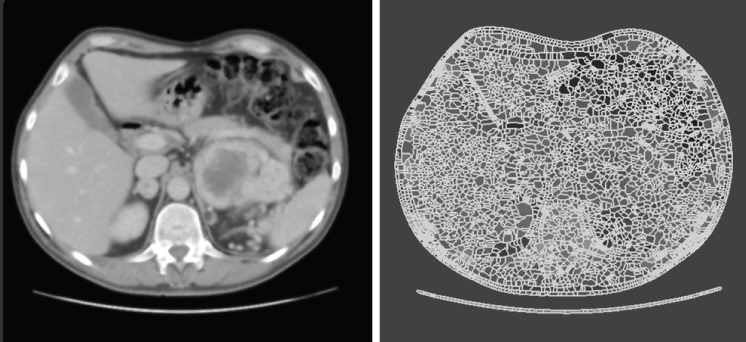
\epsfig{file=oversegmentedimage.png, height=.175\linewidth}}%
\else
        % TODO
\fi
\caption{Example of oversegmented image}
\label{fig:oversegmented}
\end{figure}
%---

Figure~\ref{fig:oversegmented} illustrates (on a CAT scan) the results
of a common segmentation algorithm, the watershed. The image is
clearly over-segmented and hence not much more useful than the
original for the purposes mentioned earlier. This over-segmented image
can be processed further by grouping together regions featuring
similar grey values. This technique is known as the {\em waterfall\/}
algorithm. It yields a partition forest hierarchy, which is a
comprehensive data structure which can be used subsequently in the
process of feature identification.
Figure~\ref{fig:waterfall} illustrates the various layers that result
from applying the waterfall algorithm repeatedly to the segmentation
shown in Figure~\ref{fig:oversegmented}.

%---
\begin{figure}
\centering
\ifpdf
        \subfigure{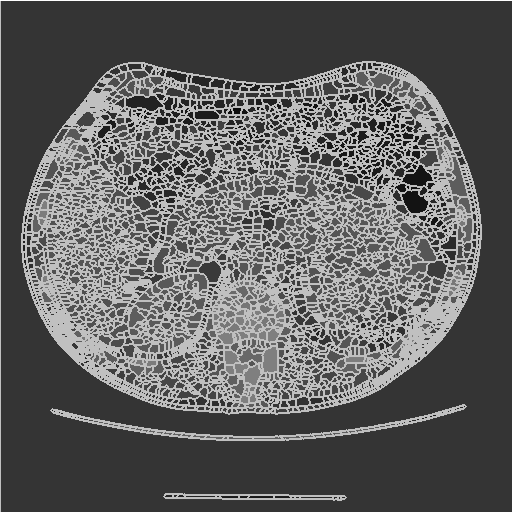
\epsfig{file=image5.png, height=.175\linewidth}}%
        \hspace{4mm}%
        \subfigure{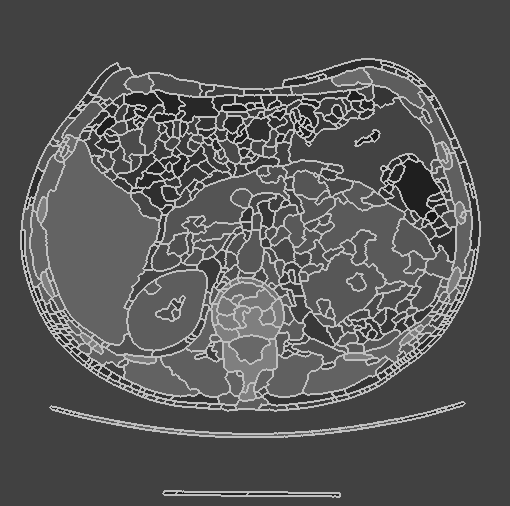
\epsfig{file=image4.png, height=.175\linewidth}}%
        \hspace{4mm}%
        \subfigure{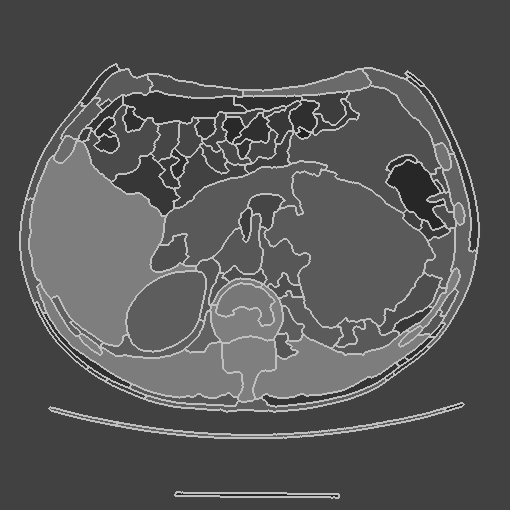
\epsfig{file=image3.png, height=.175\linewidth}}%
        \hspace{4mm}%
        \subfigure{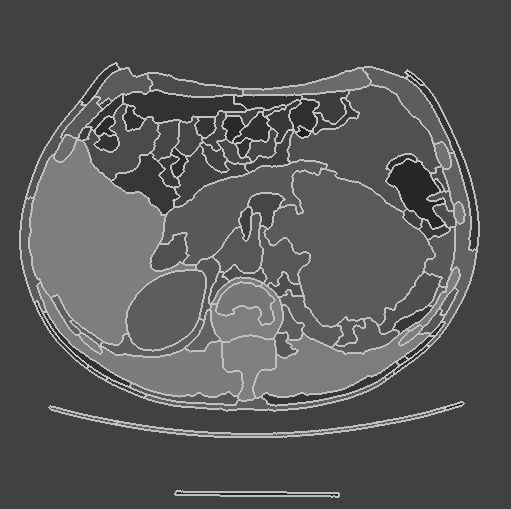
\epsfig{file=image2.png, height=.175\linewidth}}%
        \hspace{4mm}%
        \subfigure{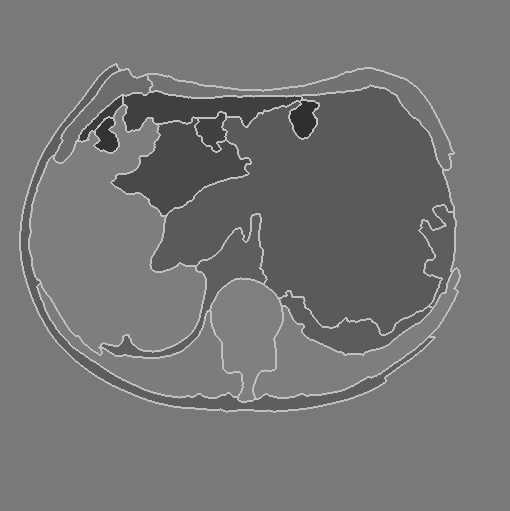
\epsfig{file=image1.png, height=.175\linewidth}}%
\else
        % TODO
\fi
\caption{Hierarchy of segmentations}
\label{fig:waterfall}
\end{figure}
%---


Both the watershed and the waterfall algorithms are based on a
geographical metaphor. The image is regarded as a landscape, with each
grey value being proportional to the terrain height. 
%
The valleys are
in the darker areas, whereas the lighter areas are regarded as peaks.

The waterfall algorithm~\cite{beucher,marcotegui} can then be imagined
as a flooding process. The water falls into (low) catchment basins and
gradually fills them up to the nearest boundaries, sometimes spilling
into adjacent regions. This process continues until the whole image
becomes a single basin. The intermediate stages of the process can be
regarded as intermediate segmentations of the image, with each basin
representing a region.

The traditional implementation of this algorithm \cite{marcotegui}
involves the construction of a Minimum Spanning Tree (MST) and the
gradual elision of some of its edges. Its nodes are the local minima
and maxima of the plateaus in the landscape, whereas its edges are the
relative difference in height between these.

The collection of regional minimum edges of a graph $G$ is a connected
subgraph of $G$ whose edges have the same weight as each other, and
whose adjacent edges in $G$ have strictly higher weights. The
waterfall algorithm relies heavily on finding these regional minimum
edges, eliding them and rebuilding the MST -- a process which not only
requires careful implementation of the MST but, more importantly, is
relatively complex and hard to implement.

In this paper we present a new data structure for the waterfall
algorithm that simplifies the process and improves efficiency compared
to current implementations. It is based on a recursive-tree data
structure and a recursive relation on the nodes rather than the
conventional iterative transformations.

The main advantage of our approach to the waterfall problem is that
the algorithm uses a single data structure (the MST) and a single loop
to walk it, which can be written in pure functional style. It walks
(bottom-up) the MST and, in a single pass, merges regions that belong
together.  The waterfall algorithm, thus improved, produces similar
layers of segmented images, combined in a hierarchical structure that
can be processed for feature identification.

Production of partition forests in this manner also has many
applications outside of the field of medical imaging, for instance,
binary space partitioning in 3D map rendering for games.



\begin{thebibliography}{2}

\bibitem{beucher}{Serge Beucher. {\em Watershed, hierarchical
    segmentation and waterfall algorithm}. In Mathematical Morphology
  and its Applications to Image Processing, Proc.\ ISMM 94, pages
  69-76, Fontainebleau, France, 1994. Kluwer Ac. Publ.}

\bibitem{marcotegui}{Beatriz Marcotegui and Serge Beucher, {\em Fast
    Implementation of Waterfall Based on Graph}. In Mathematical
  Morphology: 40 Years On, Springer Netherlands, 2005.}

\end{thebibliography}

\end{document}
